\documentclass[10pt,twoside,a4paper]{article}
% http://www-h.eng.cam.ac.uk/help/tpl/textprocessing/latex_maths+pix/node6.html symboles de math
% http://fr.wikibooks.org/wiki/Programmation_LaTeX Programmation latex (wikibook)
%=========================== En-Tete =================================
%--- Insertion de paquetages (optionnel) ---
\usepackage[french]{babel}   % pour dire que le texte est en fran{\'e}ais
\usepackage{a4}	             % pour la taille   
\usepackage[T1]{fontenc}     % pour les font postscript
\usepackage{epsfig}          % pour gerer les images
%\usepackage{psfig}
\usepackage{amsmath, amsthm} % tres bon mode mathematique
\usepackage{amsfonts,amssymb}% permet la definition des ensembles
\usepackage{float}           % pour le placement des figure
\usepackage{verbatim}

\usepackage{multicol} % multicolonnes

\usepackage{longtable} % pour les tableaux de plusieurs pages

\usepackage[table]{xcolor} % couleur de fond des cellules de tableaux

\usepackage{lastpage}

\usepackage{multirow}

\usepackage{multicol} % pour {\'e}crire dans certaines zones en colonnes : \begin{multicols}{nb colonnes}...\end{multicols} 

% \usepackage[top=1.5cm, bottom=1.5cm, left=1.5cm, right=1.5cm]{geometry}
% gauche, haut, droite, bas, entete, ente2txt, pied, txt2pied
\usepackage{vmargin}
\setmarginsrb{0.20cm}{0.20cm}{0.20cm}{0.20cm}{15pt}{3pt}{42pt}{15pt}

	
%\usepackage{frbib} % enlever pour obtenir references en anglais
% --- style de page (pour les en-tete) ---
\pagestyle{empty}

% mettre du texte en diagonale sur le fond : tikz
\usepackage{tikz} 
\def\confidentialTIKZ{%
	\begin{tikzpicture}[remember picture,overlay]
	\node[rotate=60,scale=15,text opacity=0.1] at (current page.center) {Confidentiel};
	\end{tikzpicture}
}%

\def\TIKZcyberpunkRED{%
	\begin{tikzpicture}[remember picture,overlay]
	\node[rotate=60,scale=10,text opacity=0.1] at (current page.center) {-- Cyberpunk RED};
	\end{tikzpicture}
}%

\usepackage{tikzpeople}

\def\txtTITLE{Feuille de personnage Cyberpunk RED} %%%%% !! TITRE !! %%%%%
\def\imgCORNER{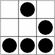
\includegraphics[width=0.25cm]{../../../../images/glider/logo-glider.png}}

\def\imgGLIDERLEFTT{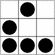
\includegraphics[width=1.95cm]{../../../../images/glider/logo-glider-left.png}}
\def\imgGLIDERRIGHT{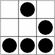
\includegraphics[width=1.95cm]{../../../../images/glider/logo-glider-right.png}}

\def\imgGLIDERLEFTTsmall{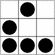
\includegraphics[width=0.25cm]{../../../../images/glider/logo-glider-left.png}}
\def\imgGLIDERRIGHTsmall{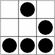
\includegraphics[width=0.25cm]{../../../../images/glider/logo-glider-right.png}}

% % % en-tete et pieds de page configurables : fancyhdr.sty

% http://www.trustonme.net/didactels/250.html

% http://ww3.ac-poitiers.fr/math/tex/pratique/entete/entete.htm
% http://www.ctan.org/tex-archive/macros/latex/contrib/fancyhdr/fancyhdr.pdf
\usepackage{fancyhdr}
\pagestyle{fancy}
	% \renewcommand{\chaptermark}[1]{\markboth{#1}{}}
	% \renewcommand{\sectionmark}[1]{\markright{\thesection\ #1}}
\fancyhf{}
\fancyhead[LE,RO]{\bfseries\thepage \TIKZcyberpunkRED }
\fancyhead[LO]{\bfseries\rightmark}
\fancyhead[RE]{\bfseries\leftmark}
\fancyfoot[LE]{\thepage /\pageref{LastPage} \hfill
	\scriptsize{\txtTITLE} % TITLE
\hfill \imgGLIDERLEFTTsmall }
\fancyfoot[RO]{\imgGLIDERRIGHTsmall \hfill
	\scriptsize{\txtTITLE} % TITLE
\hfill \thepage /\pageref{LastPage}}
\renewcommand{\headrulewidth}{0.5pt}
\renewcommand{\footrulewidth}{0.5pt}
\addtolength{\headheight}{0.5pt}
% \fancypagestyle{plain}{
	% \fancyhead{}
	% \renewcommand{\headrulewidth}{0pt}
% }

\def\smallbox{%
	\setlength{\unitlength}{0.5cm}
	\fbox{
		\begin{picture}(1, 1)(0,0)
		\end{picture}
	}
}%

%%%%%%%%%%% SOME VALUES %%%%%%%%%%%%%%%%%%%%%
\def\contentNAME{~~}
\def\contentCLASS{~~}
\def\caracINT{~~}
\def\caracREF{~~}
\def\caracDEX{~~}
\def\caracTECH{~~}
\def\caracCOOL{~~}
\def\caracWILL{~~}
\def\caracLUCK{~~}
\def\caracMOVE{~~}
\def\caracBODY{~~}
\def\caracEMP{~~}

\def\compPerception{\dotfill}
\def\compTracking{\dotfill}
\def\compEducation{\dotfill}
\def\compLocalExpert{\dotfill}
\def\compMarksmanship{\dotfill}
\def\compDriving{\dotfill}
\def\compEvasion{\dotfill}
\def\compAthletics{\dotfill}
\def\compStealth{\dotfill}
\def\compBrawling{\dotfill}
\def\compMeleeWeapon{\dotfill}
\def\compBasicTech{\dotfill}
\def\compCyberTech{\dotfill}
\def\compFirstAid{\dotfill}
\def\compBribery{\dotfill}
\def\compInterrogation{\dotfill}
\def\compPersuasion{\dotfill}
\def\compConcentration{\dotfill}
\def\compConversation{\dotfill}
\def\compHumanPerception{\dotfill}
\def\compPlayInstrument{\dotfill}
\def\compInterface{\dotfill}

\def\biographicBACKGROUND{\resizebox{0.46\linewidth}{25pt}{
\includegraphics{../../../../images/pixel.png}}}
\def\biographicMOTIVATION{\resizebox{0.46\linewidth}{25pt}{
\includegraphics{../../../../images/pixel.png}}}
\def\biographicGOALS{\resizebox{0.46\linewidth}{25pt}{
\includegraphics{../../../../images/pixel.png}}}
\def\biographicFRIENDS{\resizebox{0.46\linewidth}{25pt}{
\includegraphics{../../../../images/pixel.png}}}
\def\biographicENEMIES{\resizebox{0.46\linewidth}{25pt}{
\includegraphics{../../../../images/pixel.png}}}
\def\biographicROMANCE{\resizebox{0.46\linewidth}{25pt}{
\includegraphics{../../../../images/pixel.png}}}
\def\biographicPERSONALITY{\resizebox{0.46\linewidth}{25pt}{
\includegraphics{../../../../images/pixel.png}}}

\def\equipmentCyberWarePartOne{\resizebox{0.46\linewidth}{25pt}{
\includegraphics{../../../../images/pixel.png}} \newline \newline \newline }
\def\equipmentCyberWarePartTwo{\resizebox{0.46\linewidth}{25pt}{
\includegraphics{../../../../images/pixel.png}} \newline \newline \newline }
\def\equipmentGearPartOne{\resizebox{0.46\linewidth}{25pt}{
\includegraphics{../../../../images/pixel.png}} \newline \newline \newline }
\def\equipmentGearPartTwo{\resizebox{0.46\linewidth}{25pt}{
\includegraphics{../../../../images/pixel.png}} \newline \newline \newline }

%%%%%%%%%%% 
\definecolor{verylightred}{rgb}{1.0,0.9,0.9}
\definecolor{lightred}{rgb}{1.0,0.75,0.75}
\definecolor{red}{rgb}{1.0,0.5,0.5}

\def\CELLblackTXTWhite{\cellcolor{black} \color{white}}
\def\CELLredTXTWhite{\cellcolor{red} \color{black}}
\def\CELLwhiteTXTWhite{\cellcolor{white} \color{black}}

%============================= Corps =================================
\begin{document}

\setlength\parindent{0pt}

\begin{tabular}{ p{0.95\textwidth} }
	%% \CELLredTXTWhite
	\begin{tabular}{|p{0.20\linewidth}|p{0.75\linewidth}|} \hline
		\multirow{9}{*}{	%% \begin{tikzpicture}
							%% 	\node[maninblack,mirrored,monitor,saturated,minimum size=2.5cm]{A Corpo Rat ?};
							%% \end{tikzpicture}
							\newline \newline \newline \newline \newline \newline \newline \newline \newline 
		}
							&	Name, Classe : \contentNAME ~(\contentCLASS ) %% \framebox[0.60\textwidth][ht]{ \newline \newline }	
												\\ \cline{2-2} 
							&	\begin{tabular}{|p{0.05\textwidth}|p{0.05\textwidth}|p{0.05\textwidth}|p{0.05\textwidth}|p{0.05\textwidth}|p{0.05\textwidth}|p{0.05\textwidth}|p{0.05\textwidth}|p{0.05\textwidth}|p{0.05\textwidth}|}
									\hline
									INT						&	REF						&	DEX						&	TECH					&	COOL					&	WILL					&	LUCK					&	MOVE					&	BODY					&	EMP						\\ \hline 
									\caracINT				&	\caracREF				&	\caracDEX				&	\caracTECH				&	\caracCOOL				&	\caracWILL				&	\caracLUCK				&	\caracMOVE				&	\caracBODY				&	\caracEMP				\\ \hline
								\end{tabular}	\\ \cline{2-2}
							&					\\ \cline{2-2}
							&	\begin{tabular}{|p{0.20\textwidth}|p{0.20\textwidth}|p{0.20\textwidth}|p{0.20\textwidth}|}
									Heal Points		&	Armor SP \newline(HEAD and BODY)	&	Net Actions		&	Rep lvl	\\
								\end{tabular}	\\ \cline{2-2}
							&	\begin{tabular}{|p{0.20\textwidth}|p{0.20\textwidth}|p{0.20\textwidth}|p{0.20\textwidth}|}
													&										&					&			\\
								\end{tabular}	\\ %% \cline{2-2}
							&	\begin{tabular}{|p{0.20\textwidth}|p{0.20\textwidth}|p{0.20\textwidth}|p{0.20\textwidth}|}
													&										&					&			\\
								\end{tabular}	\\ %% \cline{2-2}
							&	\begin{tabular}{|p{0.20\textwidth}|p{0.20\textwidth}|p{0.20\textwidth}|p{0.20\textwidth}|}
													&										&					&			\\ \cline{1-4} %% \hline
								\end{tabular}	\\ %% \cline{2-2}
							&					\\ \cline{2-2}
							&					\\ \cline{2-2}
							
							&					\\ \hline
	\multicolumn{2}{ c }{ } \\
							\hline
	\multicolumn{2}{ c }{
		\begin{tabular}{|p{0.30\textwidth}|p{0.30\textwidth}|p{0.30\textwidth}|} \hline
		STARTING HITS		&		SEROUSLY WOUNDED		&	DEATH SAVE			\\ \hline
						 	&						 		&						\\ \hline
		\end{tabular}
	} \\
							 \hline
	\end{tabular}~\\~\\

	\begin{tabular}{ p{0.50\linewidth} p{0.50\linewidth} } \hline
		\footnotesize
		\begin{tabular}{|p{0.23\linewidth}|p{0.23\linewidth}|p{0.20\linewidth}|p{0.17\linewidth}|} \hline
			\textsc{\textbf{Skills}}		&	\textbf{DEX}					&	\textbf{COOL}						&	\textbf{Special}			\\ \hline
			\textbf{INT}					&	Evasion \compEvasion			&	Bribery \compBribery				&	Interface \compInterface	\\ \hline
			Perception \compPerception		&	Athletics \compAthletics		&	Interrogation \compInterrogation	&	(NetRunner)					\\ \hline
			Tracking \compTracking			&	Stealth \compStealth			&	Persuasion \compPersuasion			&								\\ \hline
			Education \compEducation		&	Brawling \compBrawling			&	\textbf{WILL}						&								\\ \hline
					 \dotfill				&	Melee Weapon \compMeleeWeapon	&	Concentration \compConcentration	&								\\ \hline
			Local Expert \compLocalExpert	&	\textbf{TECH}					&	\textbf{EMP}						&								\\ \hline
			\textbf{REF}					&	Basic tech \compBasicTech		&	Conversation \compConversation		&								\\ \hline
			Marksmanship \compMarksmanship	&	CyberTech \compCyberTech		&	Human P. \compHumanPerception		&								\\ \hline	%% Human Perception
			Driving \compDriving			&	First Aid \compFirstAid			&	Instrument \compPlayInstrument		&								\\ \hline	%% Play Instrument
		\end{tabular}
			&	
		\begin{tabular}{|p{0.27\linewidth}|p{0.27\linewidth}|p{0.27\linewidth}|}  \hline
										&							&								\\ \hline
			\textsc{\textbf{ARMOR}}		&							&								\\ \hline
										&							&								\\ \hline
			\multicolumn{3}{ c }{ } \\
			\multicolumn{3}{ c }{ } \\ \hline 
										& \textsc{\textbf{NAME}}	& \textsc{\textbf{DAMAGE}}		\\ \hline
			\textsc{\textbf{WEAPONS}}	&							&								\\ \hline
										&							&								\\ \hline
										
		\end{tabular}	\\	
		\multicolumn{2}{ c }{ } \\
		\multicolumn{2}{ c }{ } \\
		\multicolumn{2}{ c }{ } \\
		\begin{tabular}{|p{0.30\linewidth}|p{0.50\linewidth}|} \hline
			\textsc{\textbf{Background}}	&	\biographicBACKGROUND		\\ \hline
			\textsc{\textbf{Motivation}}	&	\biographicMOTIVATION		\\ \hline
			\textsc{\textbf{Goals}}			&	\biographicGOALS			\\ \hline
			\textsc{\textbf{Friends}}		&	\biographicFRIENDS			\\ \hline
			\textsc{\textbf{Ennemies}}		&	\biographicENEMIES			\\ \hline
			\textsc{\textbf{Romance}}		&	\biographicROMANCE			\\ \hline
			\textsc{\textbf{Personnality}}	&	\biographicPERSONALITY		\\ \hline
			\multicolumn{2}{ c }{ } \\
			\multicolumn{2}{ c }{ } \\
			\multicolumn{2}{ c }{ } \\
			\multicolumn{2}{ c }{ } \\
			\multicolumn{2}{ c }{ } \\
			%% 								&	\resizebox{0.46\linewidth}{25pt}{
\includegraphics{../../../../images/pixel.png}}	\\ 
		\end{tabular}
			&
		\begin{tabular}{|p{0.46\linewidth}|p{0.46\linewidth}|} \hline
			\textsc{\textbf{CYBERWARE}}		&	\textsc{\textbf{GEAR}}			\\ \hline
				\equipmentCyberWarePartOne	& 	\equipmentGearPartOne			\\ \hline
				\equipmentCyberWarePartTwo	& 	\equipmentGearPartTwo			\\ \hline
		\end{tabular}	\\
	
	\end{tabular}
\end{tabular}

\end{document}
